% Preamble
% ---
\documentclass{article}


% Packages
% ---
%\usepackage{amsmath} % Advanced math typesetting
\usepackage[utf8]{inputenc} % Unicode support (Umlauts etc.)
\usepackage[ngerman]{babel} % Change hyphenation rules
\usepackage{hyperref} % Add a link to your document
\usepackage{graphicx} % Add pictures to your document
\usepackage{listings} % Source code formatting and highlighting
\usepackage{caption}
\usepackage{subcaption}

\graphicspath{ {./img/} }

\begin{document}

    \author{Federico Rachelli}
    \title{\vspace{-2cm}DataVirus.it}
    \maketitle
    
    \section{Funzionamento dell'applicazione}

    L'app \textbf{\href{https://datavirus.it}{DataVirus.it}} é ispirata dal sito web omonimo.
    Fornisce all'utente una visualizzazione grafica dei dati del Dipartimento di Protezione Civile sull'andamento dell'epidemia di COVID-19.
    \\
    I dati sono accedibili dal \href{https://github.com/pcm-dpc/COVID-19}{repository GitHub ufficiale} della Protezione Civile. 
    Tali dati sono aggiornati quotidianamente (a partire dalle ore 18:00) fino alla fine dello stato di emergenza dichiarato dal Consiglio dei Ministri in data 31 Gennaio 2020.
    
    \subsection{Visualizzazione dati numerici}
    L'applicazione all'avvio visualizza una schermata di caricamento dei dati dal Dipartimento di Protezione Civile. 
    Tali dati, una volta ottenuti, sono elaborati e vengono mostrati all'utente gli andamenti a livello nazionale dell'epidemia.
    
    \begin{figure}[h]
        \centering
        \begin{subfigure}{.5\textwidth}
          \centering
          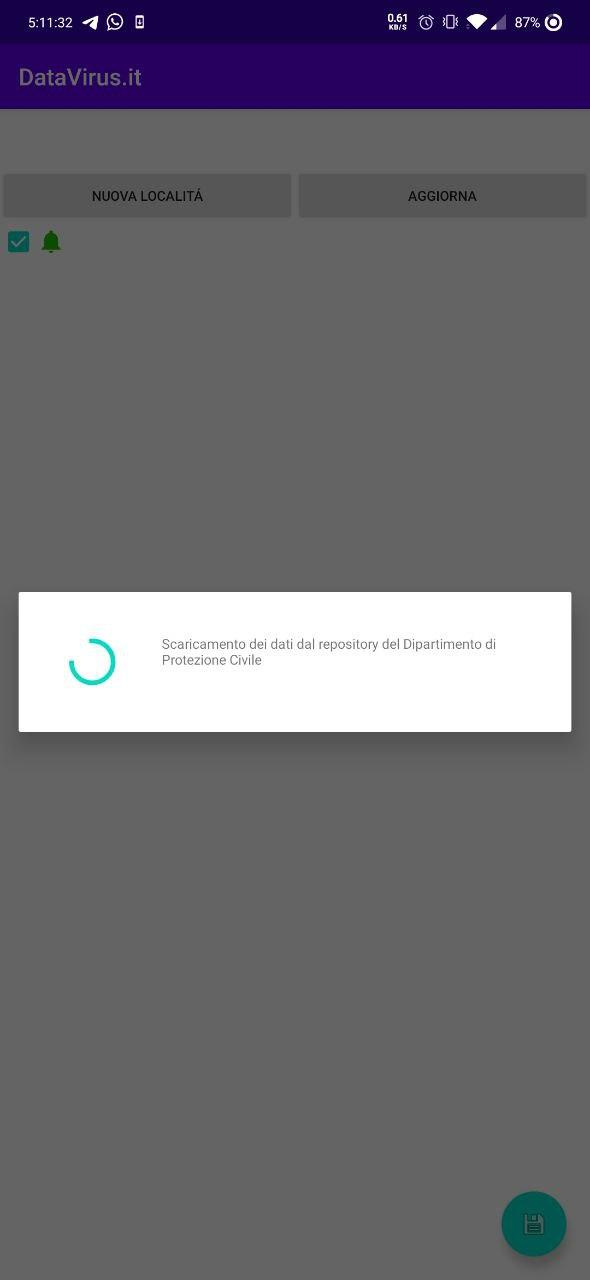
\includegraphics[width=.7\linewidth]{loading_dialog.jpg}
          \caption{Caricamento dei dati}
          \label{fig1:sub1}
        \end{subfigure}%
        \begin{subfigure}{.5\textwidth}
          \centering
          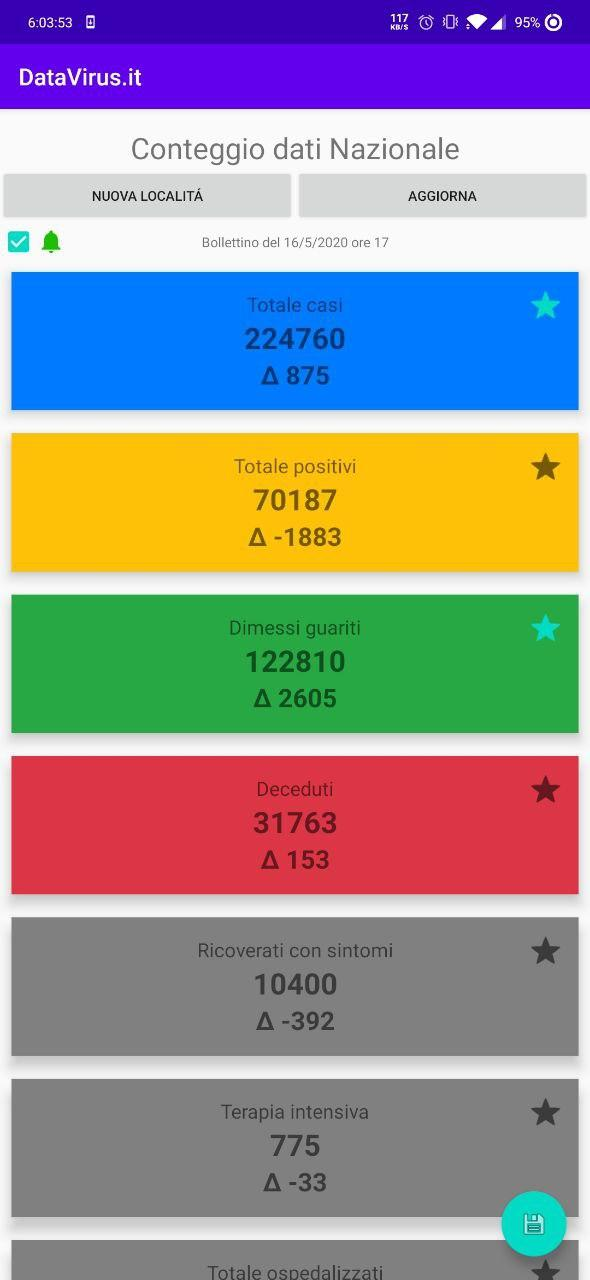
\includegraphics[width=.7\linewidth]{main_activity.jpg}
          \caption{Andamento nazionale}
          \label{fig1:sub2}
        \end{subfigure}
        %\caption{A figure with two subfigures}
        % \label{fig:test}
    \end{figure}
    
    Come si puó notare nella figura \ref{fig1:sub2}, questa é la schermata principale dell'applicazione. 
    Viene mostrato in alto la denominazione territoriale dei dati (nella scermata principale verrá mostrato l'andamento nazionale). Sotto i pulsanti, viene visualizzata la data dell'ultimo aggiornamento disponibile dal Dipartimento di Protezione Civile.
    \\
    Il pulsante "Aggiorna" ricarica i dati dal repository.
    \\
    Vengono poi visualizzate le tile contenenti il dato odierno e la relativa variazione (delta) rispetto alla giornata precedente.
    \\
    Ogni tile ha in alto a destra una \emph{stellina}: quando premuta, la tile relativa viene salvata tra i preferiti.
    Per recuperare la lista delle tile salvate é sufficiente premere sul floating button in basso a destra (visibile nella schermata principale dell'app).

    \begin{figure}[h]
        \centering
        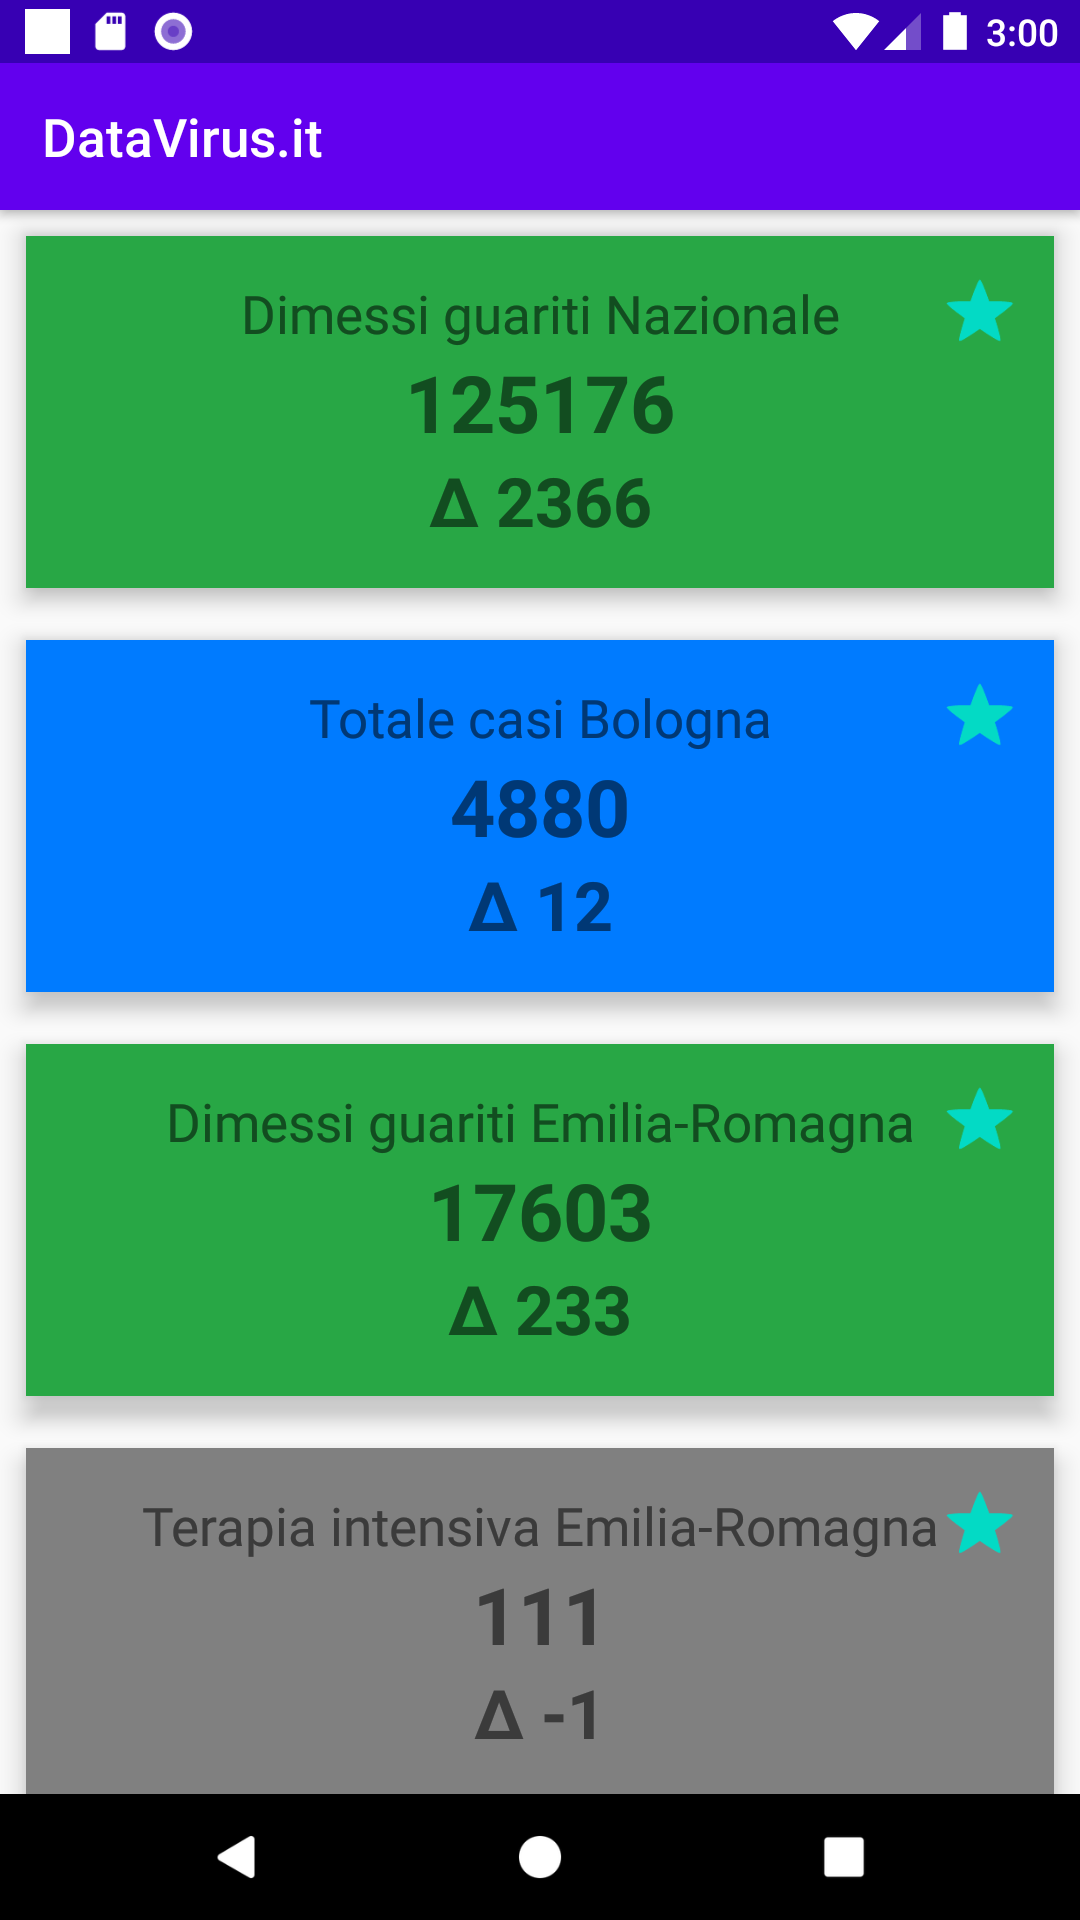
\includegraphics[width=.5\linewidth]{preferences.png}
        \caption{Lista dei preferiti}
        \label{fig2}
    \end{figure}

    Come si puó notare dalla figura \ref{fig2}, le tile salvate sono visualizzate con la loro denominazione geografica a seguito.

    \subsection{Cambio zona geografica}
    La denominazione geografica puó essere cambiata premendo sul pulsante "Nuova localitá" dalla schermata principale (vedi \ref{fig1:sub2}).
    \\
    Appare il picker della zona geografica:

    \begin{figure}[h]
        \centering
        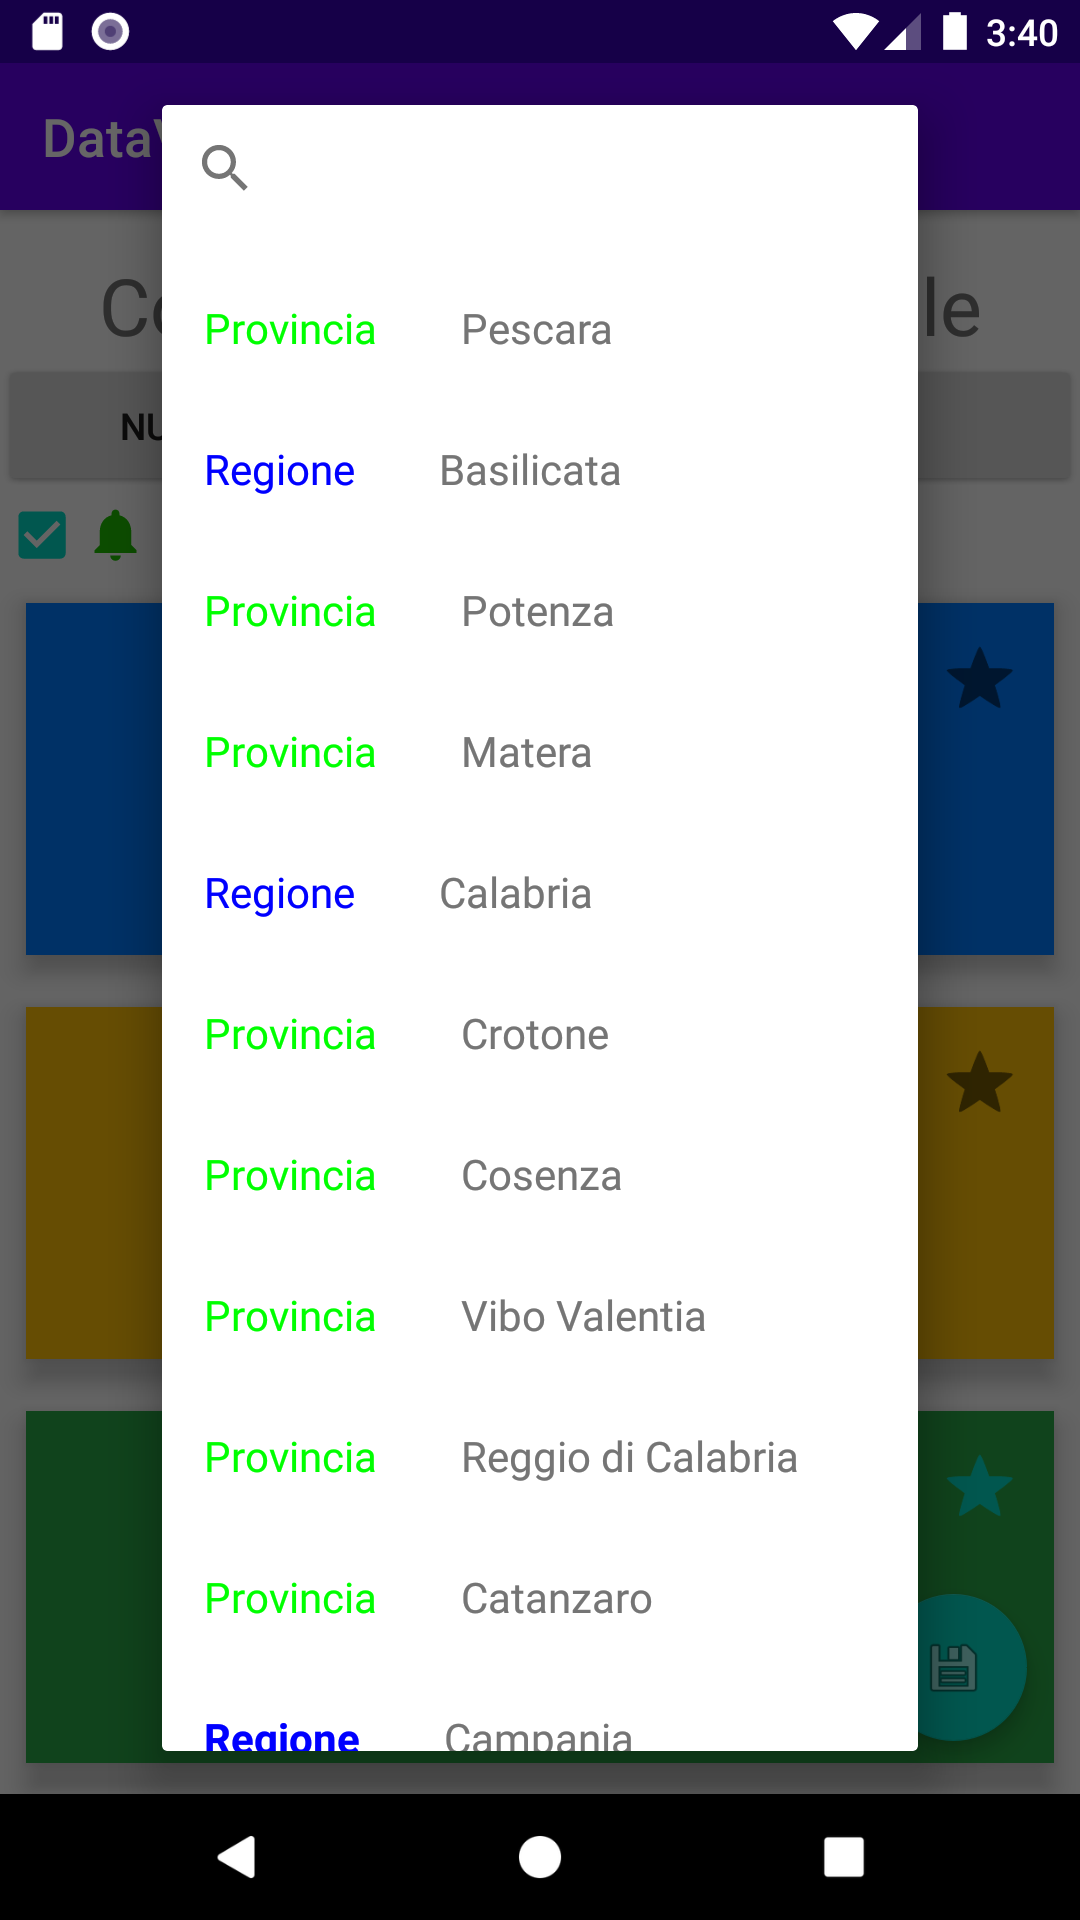
\includegraphics[width=.5\linewidth]{DPC_geo_picker.png}
        \caption{Picker zona geografica}
        \label{fig3}
    \end{figure}

    Grazie al picker si puó scegliere la zona geografica di interesse. Puó essere una provincia, una regione oppure si puó selezionare l'andamento nazionale.
    Per comoditá si puó ulteriormente cercare la zona d'interesse grazie al pulsante in alto con la \emph{lente d'ingrandimento}.


\end{document}